\MakeShortVerb{\|}
\label{sec:choices}

One important questions of this project is to find a suite of relevant
frameworks in order to work with testing in a Rails application, and
gather experience with working with these. This subsection presents our
evaluation of the different frameworks and tools used for testing.\\

The choice of frameworks for development was mainly given by the
constituent, since the existing software was written in Ruby on Rails
with KnockoutJS and a MongoDB database. The main server-side language
was thus Ruby, and the client-side code was written in CoffeeScript.
CoffeeScript is a scripting language which compiles into Javascript.\\

For the choice of testing-related frameworks, we chose to look for
frequently used and active developed open source frameworks.
Technologies that are used by many people intuitively often has more
resources on how they are used, and also has the advantage of being more
likely to be recognized by future developers. Active development of used
frameworks is crucial, most importantly since they are likely to be
incompatible with future versions of other frameworks (such as Rails).
Another benefit is that new features and bug fixes are released. The
Ruby Toolbox website \footnote{\url{https://www.ruby-toolbox.com/}},
which uses information from the Github and RubyGems websites, was
consulted in order to find frameworks with mentioned qualities.\\

\subsection{Ruby test frameworks and tools}

\label{sec:ruby_test}

Before the case study, Cucumber\footnote{\url{http://cukes.info/}} and
RSpec\footnote{\url{http://rspec.info/}} were used as testing frameworks
for existing tests. We evaluated these frameworks, as well as considered
new frameworks in the beginning of the case study.\\

\subsubsection{Cucumber}

We worked with Cucumber during the first part of the case study, since
the major part of all existing tests was written using this framework.
Cucumber is a framework for acceptance-level testing using BDD
methodology. Tests, called \emph{features}, are written using an
ubiquitous language as seen in listing \ref{lst:cucumber_feature}. The
action for each line, called \emph{step}, of the feature is specified
using a \emph{step definition}, as seen in listing
\ref{lst:cucumber_step}.\cite{web:cucumber}\\

One benefit from using Cucumber is that all steps are reusable, which
means that code duplication can be avoided. However, it can be hard to
write the steps in such way that they benefit from this, and it
sometimes also requires a lot of parameters to be passed in to each
step. Cucumber also provides code snippets for creating step
definitions, which evades some unnecessary work.\\

Apart from these benefits, we found Cucumber tiresome to work with. The
separation between features and step definitions makes it hard to get an
overview of the code executed during the test, and it is often hard to
find specific step definitions. We also experienced problems with the
mapping step definitions, where the generated step definition simply did
not match the written step.\\

The chosen level of testing is another big issue. We felt that using
TDD-methodology was hard to do with system-level tests since they take
long time to execute and affects a much larger part of the software than
the part we are typically working with when implementing new
functionality. Considering these drawbacks, we decided to not continue
the use of Cucumber for this thesis.\\


\begin{lstlisting}[caption=Example of a Cucumber test.,
                   label=lst:cucumber_feature, float=t, language=HTML]
Feature: creating new cookies
  As a bakery worker
  So that I can sell cookies to my customers
  I want to create a new cookie object

Background:
  Given a user and a cookie type called "Chocolate chip"
  And I have created one cookie

Scenario: create a new cookie
  When I visit the page for creating cookies
  Then I should see one cookie
  When I create a new Chocolate chip cookie
  Then I should see two cookies
\end{lstlisting}


\begin{lstlisting}[caption=Cucumber step definition for the step on row 13 in code listing \ref{lst:cucumber_feature}.,
                   label=lst:cucumber_step, float=t]
When /^I create a new (.+) cookie$/ do |cookie_type|
  # Code for creating a new cookie
end
\end{lstlisting}


\subsubsection{RSpec}

Just like Cucumber, RSpec also claims to be made for use with
BDD \cite{web:rspec}. In contrast, it only uses descriptive strings
instead of a full ubiquitous language and can be used for writing
isolated unit tests as well as integration- and browser tests.\\

As an alternative to RSpec, we also considered
Minitest\footnote{\url{https://github.com/seattlerb/minitest}}. Similar
to RSpec, Minitest is popular as well as actively developed. In contrast
to RSpec, it is more modular and claims to be more readable. It also
claims to be more minimalistic and lightweight. By looking at code
examples and documentation, we however found that the syntax of the
tests for recent versions of both these frameworks seemed to be very
similar. We did not find any considerable advantages of using Minitest
over RSpec and therefore concluded that RSpec was a better option, since
some of the existing tests already was written using this framework and
migrating these would require additional work.\\

We found it quite straightforward to write tests using RSpec, and to use
descriptive strings rather than function names for describing tests as
seen in code listing \ref{lst:rspec}. The plug-in rspec-mocks\footnote{\url{https://github.com/rspec/rspec-mocks}}
were used in
some situations where mocking was required, since the RSpec core package does
not include support for this. One major drawback of rspec-mocks is that
it allows stubbing non-existent methods and properties, which as
discussed in \fref{sec:theory_mocks} can be dangerous. We worked around
this by writing a helper for checking existence of properties before
stubbing them.\\

\begin{lstlisting}[caption=Example of RSpec tests for a module.,
                   label=lst:rspec, float=t]
describe Math do
  describe '#minus' do
    it 'returns the difference between two positive integers' do
      expect(Math::minus(3, 1)).to(eq(2))
    end

    it 'returns the sum if the second integer is negative' do
      expect(Math::minus(5, -2)).to(eq(7))
    end
  end

  describe '#plus' do
    it 'returns the sum of two positive integers' do
      expect(Math::plus(1, 2)).to(eq(3))
    end
  end
end
\end{lstlisting}


\subsubsection{Factory girl}
\MakeShortVerb{\|}

One important framework used was
factory\_girl\footnote{\url{https://github.com/thoughtbot/factory\_girl}},
which is used for generating factory objects. As discussed in
\fref{sec:theory_mocks}, factory objects behaves just like instances of
model objects, but has several advantages. As alternatives to
factory\_girl, we also considered
Machinist\footnote{\url{https://github.com/notahat/machinist}} and
Fabrication\footnote{\url{http://www.fabricationgem.org/}}. Machinist
was discarded since it is no longer actively developed. We did not find
any significant differences between Fabrication and factory\_girl, and
therefore chose the latter since it was more popular.\\

There are many advantages of using a framework such as factory\_girl
rather than just instantiate model objects by hand (i.e. just write
|MyModel.new| in Ruby to create a new model instance). First of all,
factory\_girl automatically passes in default values for required
parameters, so that we only need to supply the attributes needed in a
particular test. Secondly, related objects are also created
automatically, which typically saves as huge amount of work compared to
manual creation of objects. Code listing \ref{lst:factory_def} and
\ref{lst:factory_use} shows a factory definition and its usage. The name
of the cookie and a new Bakery-object is created automatically since we
do not give them as parameters when using the factory.\\

We did initially have some issues with the creation of related objects
since the factory\_girl documentation did not cover working with
document-based databases such as MongoDB in our case, but we eventually
found out how to do this.\\

One feature that we felt was missing in factory\_girl was the ability to
specify attributes on related objects, for example to specify the name
of a Bakery when creating a new Cookie. It is of course possible to
first create a Bakery object and then creating a Cookie and pass in the
created bakery object, but a shortcut for doing this would have been
convenient in some situations. To our knowledge, Fabrication also lacks
this feature.\\

\begin{lstlisting}[caption=Example usage of the factory defined in code listing \ref{lst:factory_def}.,
                   label=lst:factory_use, float=t]
FactoryGirl.create :cookie, diameter: 4.5, thickness: 0.5
\end{lstlisting}

\begin{lstlisting}[caption=A factory definition for a Cookie model.,
                   label=lst:factory_def, float=t]
FactoryGirl.define do
  factory :cookie do
    name      'Vanlilla dream'
    diameter  1
    thickness 2
    bakery    { FactoryGirl.build(:bakery) }
  end
end
\end{lstlisting}



\subsubsection{Other tools}

TimeCop\footnote{\url{https://github.com/travisjeffery/timecop}} was
used in order to mock date and time for a test that was dependent on the
current date and time. We do not have much experience from using this
tool, but it worked as we expected for our specific use.\\


\subsection{Frameworks for browser-testing}
Capybara and site\_prism.

\subsubsection{Selenium 2}
The absolutely most widespread framework for browser testing seems to be
Selenium\footnote{\url{http://docs.seleniumhq.org/}}. In fact, we have
not even been able to find any other frameworks for running tests in
real browsers, possibly since it takes a lot of effort to integrate with
a large number of browsers on a large number of platforms. Selenium
supports a number of popular programming languages, for example Java,
C\#, Python and Ruby, and also has support the majority of all modern web
browsers on Windows as well as Linux and Mac OS. The interface used by
newer versions of Selenium for interacting with browsers, WebDriver, has
been proposed as an W3C Internet
standard\footnote{\url{https://dvcs.w3.org/hg/webdriver/raw-file/default
/webdriver-spec.html}}, which may indicate that support for Selenium
will be continue to be present in future browser versions.
\cite{wiki:selenium}\\

While Selenium is very widespread and seems to be the only option for
running tests in real browsers, its API is on a rather low level. In
order to fill in a string of text to a text field, we have to locate the
label of the field using an XPath\footnote{XPath is a language for
selecting elements and attributes in an XML document, such as an
website.} function, then figure out its associated text element and
sending out text as keystrokes to this element. Rather than writing
helper methods for such functionality ourselves, we decided to use
a higher-level framework.\\


\subsubsection{Capybara}
Capybara\footnote{\url{https://github.com/jnicklas/capybara}} provides a
much higher level API for browser testing compared to Selenium, and
besides from using it with Selenium it can also be used with drivers for
headless browsers or for testing frameworks using mock requests. Tests
can also be written in multiple testing frameworks, such as RSpec which
was used in our case.\\

We did not find any particular difficulties when using Capybara. Its API
provides very convenient high-level helpers for every common task that
we needed, and we did not experience any problems with any of them. An
example of a browser test using Capybara is found in code listing
\ref{lst:capybara}.\\


\begin{lstlisting}[caption=A browser test written in RSpec using Capybara.,
                   label=lst:capybara, float=t]
describe 'creating new cookies' do
  before do
    FactoryGirl.create :cookie_type, name: 'Chocolate chip'
    login_as FactoryGirl.create :user
  end

  it 'should be possible to create new cookies' do
    visit new_cookie_path

    fill_in 'Amount', with: 1
    select 'Chocolate chip', from: 'Cookie type'
    click_button 'Save'

    expect(page).to have_content 'The cookie has been created.'
  end
end
\end{lstlisting}


\subsubsection{SitePrism}

As mentioned in \fref{sec:testing_web}, one way of writing more
structured browser tests is to use the page object pattern. We chose to
use this pattern from the start rather than cleaning up overly
complicated tests afterwards. While this pattern is perfectly possible
to use without any frameworks, we found a framework called
SitePrism\footnote{\url{https://github.com/natritmeyer/site_prism}}
which provided some additional convenient functionality.\\

SitePrism makes it possible to define pages of an application by
specifying its URL, as well as elements and sections of a specific page
by specifying a CSS or XPath selector. An example of a such definition
can be seen in code listing \ref{lst:siteprism_page}. Page objects
automatically gets basic methods for accessing elements, and allows us
to define additional methods for each page or element. This allows us to
use higher-level functions in our tests rather than locating elements
manually in out Capybara tests, as seen in code listing
\ref{lst:siteprism_test}.\\

One drawback of using SitePrism can be that elements currently must be
specified using selectors rather than having the possibility to select
them based on text, which is possible with Capybara directly. On the
other hand, it would be trivial to create a method for doing this. Using
text for locating elements also only makes sense for some specific
cases. Overall, we found the page object pattern as well as SitePrism
very convenient to work with.\\

\begin{lstlisting}[caption=Page definition for a page with a list of cookie information.,
                   label=lst:siteprism_page, float=t]

class CookieRowSection < SitePrism::Section
  element :name, '.name'
  element :amount, '.amount'
end

class CookiePage < SitePrism::Page
  set_url '/cookies'

  element :heading, 'h1'
  element :new_cookie_button, 'button#createCookie'
  sections :cookies, CookieRowSection, '.cookieInfo'

  def create_cookie
    self.new_cookie_button.click
  end
end

\end{lstlisting}

\begin{lstlisting}[caption=Browser test using SitePrism a page object defined in
                           code listing \ref{lst:siteprism_page}.,
                   label=lst:siteprism_test, float=t]

describe 'cookie information page' do
  before do
    FactoryGirl.create :cookie, name: 'Vanilla dream', amount: 2
    FactoryGirl.create :cookie, name: 'Apple crush', amount: 4
    @cookie_page = CookiePage.new
    @cookie_page.load
  end

  it 'should contain a list of cookies in alphabetical order' do
    expect(page.heading.text).to eq('List of cookies')
    expect(page.cookies.length).to be(2)

    cookie = page.cookies.first
    expect(cookie.name.text).to eq('Apple crush')
    expect(cookie.amount.text).to eq('2')
  end
end

\end{lstlisting}


\subsection{Javascript test frameworks}

\label{sec:js_test}

There are a few different frameworks for testing Javascript or
CoffeeScript code. We had previously good experiences from working with
Jasmine\footnote{\url{http://jasmine.github.io/}}. We also found that
this framework seemed to be very popular, actively developed and had
good documentation\footnote{It is worth to mention that the Jasmine
documentation is basically its own test suite with some additional
comments. This works incredibly good in this case, presumably since it
is a testing framework and the tests are very well-written.}. Code
listing \ref{lst:jasmine} shows an example of a Jasmine test written in
CoffeeScript. The syntax of Jasmine is inspired by RSpec, which is
another advantage since RSpec is used for the server side tests.\\

\subsubsection{Test runner}

The Jasmine framework provides a way of writing tests, but a test runner
is also required in order to run the tests. Jasmine ships with a basic
test runner, which was used initially and worked natively using
the Jasmine Ruby gem. A screenshot of this test runner is shown in
\fref{fig:jasmine_runner}.\\

\begin{figure}
\centering
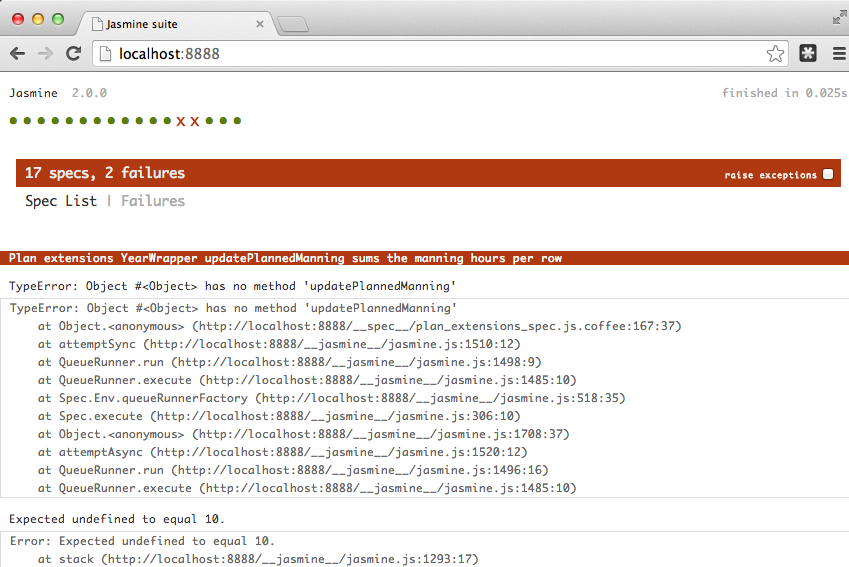
\includegraphics[width=0.8\textwidth]{results/choices/jasmine_runner}
\caption{The test runner bundled with Jasmine.}
\label{fig:jasmine_runner}
\end{figure}

The Jasmine test runner did however have multiple issues. First of all,
it runs completely in the browser. Switching to the browser and reload
the page in order to run the tests are not excessively problematic, but
might be tiresome in the long run when using a test-driven development
methodology.\\

A larger problem with the default test runner was that the asset
handling, i.e. the process of compiling CoffeeScript into Javascript.
Rails handles this compilation upon each reload when using the Jasmine
gem. Since the used version of Rails re-compiles all assets upon page
load if any file has been changed, this process takes a while, which
means that each test run could take up to 10-15 seconds even though the
actual tests only takes a fraction of a second to run. The asset
compilation also got stuck for apparently no reason once in a while.
Since the server port on which the test runner runs cannot be specified,
it is also impossible to restart the test runner without manually
killing its system process.\\

Another issue with the Jasmine test runner is that syntax errors are
printed in the terminal rather than in the browser window where the test
result is reported, which is confusing. In practice, syntax errors were
often undetected for a long time, which required more debugging than
necessary.\\

Due to these issues, we switched to the Karma\footnote{\url{http
://karma-runner.github.io/}} test runner. Karma originates from a
master's thesis by \citet{article:karma}, which covers several problems
with the Jasmine test runner as well as with some other Javascript test
runners. Karma was designed to solve several of these issues and to be
used with test-driven software methodologies. Tests are run in a browser
as soon as a file is changed, and the results are reported back to the
terminal and displayed as shown in \fref{fig:karma_runner}. Re-
compilation of source files and tests is very fast and we did not
experience any stability issues. One minor drawback is however that
pending tests is not displayed very clearly. This can be solved by using
a different Karma test reporter.\\

It took some effort getting Karma to work with Rails, since Karma is
written in Node.js and does not have any knowledge about which
CoffeeScript files that exist in the Rails application. The task of
finding the location of all such files became more complex since
external Javascript libraries such as jQuery was loaded as Ruby gems,
and therefore not even located inside the project folder. We ended up
using a slightly modified version of a Rake script from a blog entry by
\citet{web:saunier_angular} for bootstrapping Karma in a Rails
environment. This script basically collects a list of filenames for all
Javascript assets by using Rails internal modules for asset handling,
and injects it into Karma's configuration file.\\

After the case study, we discovered another Javascript test runner
called Teaspoon\footnote{\url{https://github.com/modeset/teaspoon}},
which is built for Rails and can discover assets by default. We believe
that this test runner looks very promising and may be more suitable for
Rails projects than Karma. At the time of this writing, Teaspoon does
not have support for the most recent version of Jasmine and therefore
does not work with our test suite. We were thus unable to evaluate
Teaspoon any further.\\

\begin{lstlisting}[caption=Example of Jasmine tests for a module (compare with code listing \ref{lst:rspec}).,
                   label=lst:jasmine, float=t, language=HTML]
describe 'Math', ->
  describe 'minus', ->
    it 'returns the difference between two positive integers', ->
      expect(Math.minus(3, 1)).toEqual(2)

    it 'returns the sum if the second integer is negative', ->
      expect(Math.minus(5, -2)).toEqual(7)

  describe 'plus', ->
    it 'returns the sum of two positive integers', ->
      expect(Math.plus(1, 2)).toEqual(3)
\end{lstlisting}

\begin{figure}
\centering
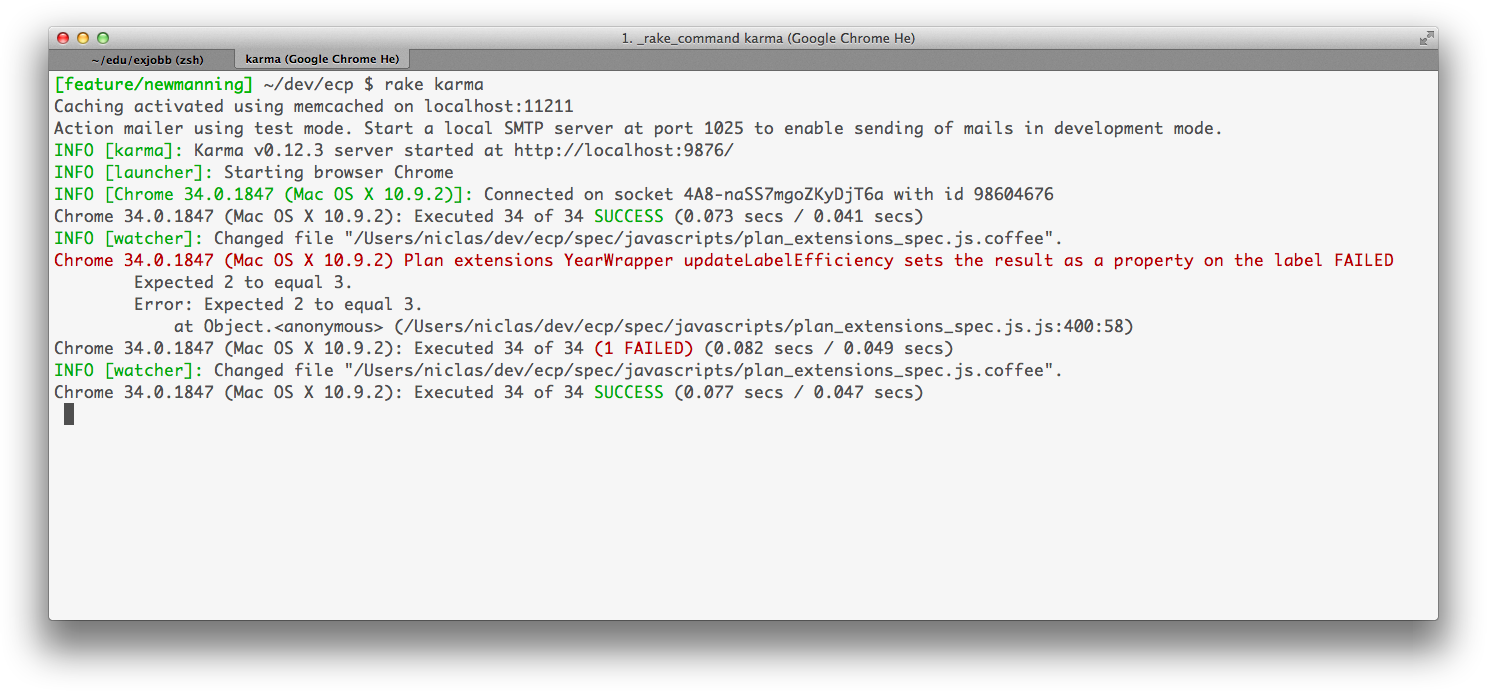
\includegraphics[width=0.8\textwidth]{results/choices/karma_runner}
\caption{The Karma test runner.}
\label{fig:karma_runner}
\end{figure}


\subsection{Test coverage}
\label{sec:coverage_frameworks}

\subsubsection{Ruby test coverage}
There are multiple different ways of analyzing test coverage, and the
properties and conditions for each different kind of test coverage are
discoursed in \fref{sec:coverage}. However, we were unable to find any
test coverage tools for Ruby which analyzed anything else than statement
coverage, which is the weakest test coverage metric. Quite much effort
was spent on finding such tool, but without any success. Several
websites and Stack Overflow-answers indicate that no such tool exists
for Ruby at the time of this writing \cite{web:coverage_ruby19,
so:c1c2_coverage, so:c1_coverage, web:toolbox_code_metrics}. On one
hand, some of these sources are rather old and might be outdated, which
would indicate that such tool could have been created recently. On the
other hand would at least some of these sources probably been updated if
such tool became available.\\

We ended up using the
SimpleCov\footnote{\url{https://github.com/colszowka/simplecov}} tool
for Ruby test coverage metrics. At the time of this writing, it is the
most used Ruby tool for test coverage. It is also actively developed,
works with recent Ruby versions and RSpec versions, and produces pretty
and easy- to-read coverage reports in HTML (see
\fref{fig:simplecov_report}). \cite{web:toolbox_code_metrics}\\

\begin{figure}
\centering
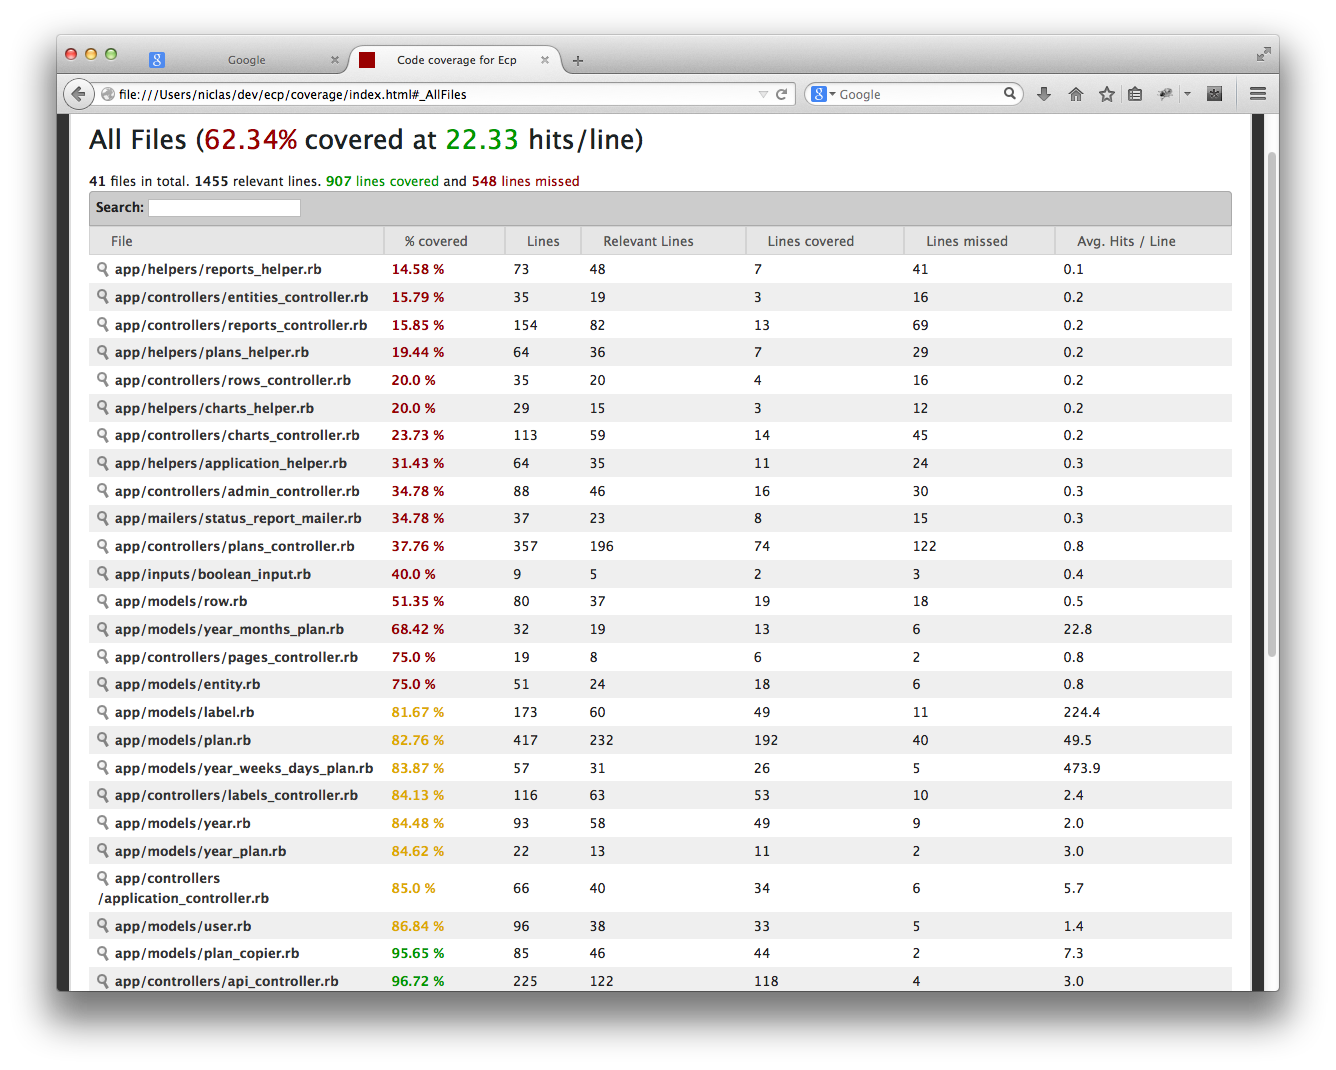
\includegraphics[width=0.8\textwidth]{results/choices/simplecov}
\caption{A test coverage report generated by SimpleCov.}
\label{fig:simplecov_report}
\end{figure}


\subsubsection{CoffeeScript test coverage}
For the client-side CoffeeScript, we used a plug-in for the Karma test
runner called karma-coverage\footnote{\url{https://github.com/karma-
runner/karma-coverage}}. This tool basically integrates Karma with
Ibrik\footnote{\url{https://github.com/Constellation/ibrik}}, which is a
tool developed by Yahoo! for measuring test coverage of CoffeeScript
code. We did initially have some problems with getting this tool to work
correctly, since Ibrik internally uses another CoffeeScript compiler;
CoffeeScriptRedux, than the compiler used when tests itself are run.
CoffeeScriptRedux is more strict and yielded syntax errors in some of
our files, which could be compiled correctly in the production code. The
latest available release of Ibrik (version 1.1.1) also had major issues
with certain constructs in CoffeeScript, which made the files impossible
to analyze. These issues were however fixed in the development version.
Ibrik was first released in December 2013, which may explain its
immaturity. Ibrik internally uses istanbul-js for the coverage
analysis and report generation.\\

The chosen solution worked very well after sorting out the issues.
Statement coverage as well as branch coverage is supported, and it
yields useful reports. As with SimpleCov, the coverage reports are
produced as an interactive HTML report (see \fref{fig:karma_report}).\\

\begin{figure}
\centering
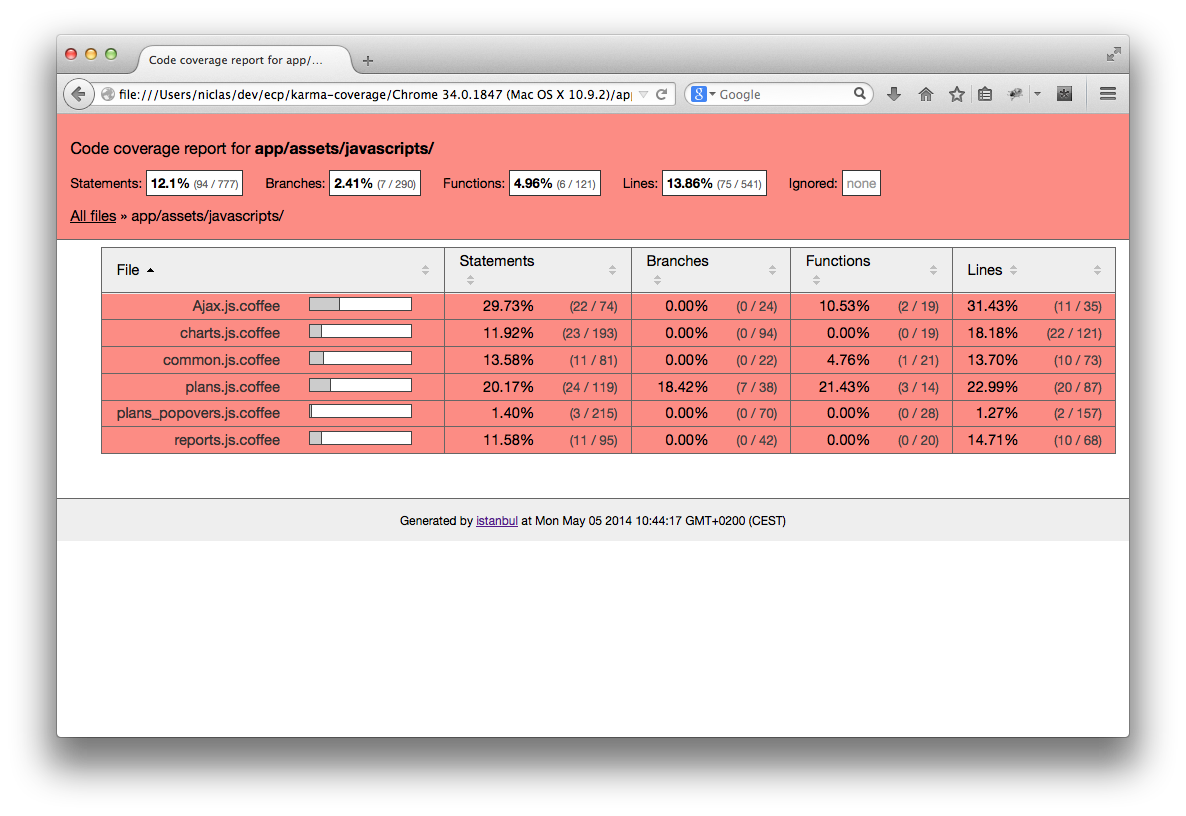
\includegraphics[width=0.8\textwidth]{results/choices/karma_coverage}
\caption{A test coverage report generated by istanbul-js using karma-coverage.}
\label{fig:karma_report}
\end{figure}


\subsubsection{Test coverage issues}

One issue with using test coverage in this particular project is the
fact that very few files were added. Most of the changes were made in
existing classes and files, either as new functions or as changes to
existing functions. Since the overall test coverage is measured per
file, it is impossible to get an exact measure of how well tested the
new and refactored code is, since old and completely untested code
lower the test coverage.\\

We have tried to mitigate this by looking at the coverage reports by
hand, and try to determine a subjective measure of how good the test
coverage is for new and refactored code. \Fref{fig:coverage_example}
shows an excerpt of a coverage report. In this case, our subjective
measure would say that the function |exports.getProduction()| is
completely untested. The function |exports.getLabelId()| is well tested
and has full statement- as well as branch coverage. The function
|exports.formatValues()| has full statement coverage, but non-optimal
branch coverage since the cases where |x| or |y| is not set are not
covered.\\

\begin{figure}
\centering
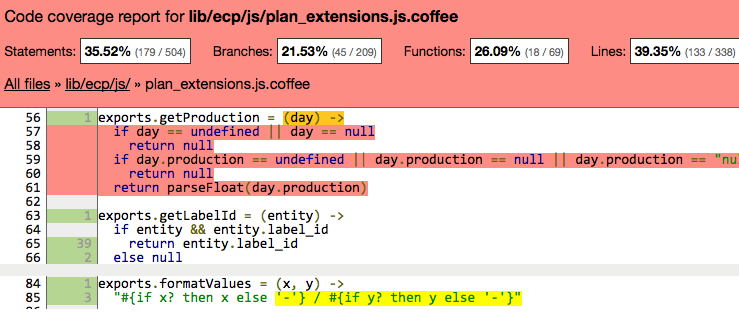
\includegraphics[width=0.8\textwidth]{results/choices/js_coverage}
\caption{An excerpt from a coverage report generated using karma-coverage
         which demonstrates three different types of tested functions.}
\label{fig:coverage_example}
\end{figure}


\subsection{Mutation analysis}
An alternative to draw conclusions from which paths of the code that is
run by a test, as done when using test coverage, is to draw conclusions
from what happens when we modify the code. The idea is that if the code
is incorrect, the test should fail. Thus, we can modify the code so it
becomes incorrect and then look at whether the test fails or not.\\

Mutation testing is done by creating several versions of the tested
code, where each version contains a slight modification. Each
such version containing a mutated version of the original source code is
called a \emph{mutant}. A mutant only differs at one location compared
to the original program, which means that each mutant should represent
exactly one bug.\cite{article:mutation, wiki:mutation}\\

\begin{lstlisting}[caption=Example of a piece of code before mutation,
                   label=lst:mutation_before, float=t]
    def odd?(x, y)
        return (x % 2) && (y % 2)
    end
\end{lstlisting}


\begin{lstlisting}[caption=Mutated versions of \ref{lst:mutation_before},
                   label=lst:mutation_after, float=t]
    def odd?(x, y)
        return (x % 2) && (x % 2)
    end

    def odd?(x, y)
        return (x % 2) || (y % 2)
    end

    def odd?(x, y)
        return (x % 2) && (0 % 2)
    end

    def odd?(x, y)
        return (x % 2)
    end
\end{lstlisting}

There are numerous ways of creating mutations to be used in mutants. One
could for example delete a method call or a variable, exchange an
operator for another, negate an if-statement, replace a variable with
zero or null-values, or something else. Code listing
\ref{lst:mutation_before} shows an example of a function which should
return true if both arguments are odd. Several mutated versions of this
example is shown in code listing \ref{lst:mutation_after}. The goal of
each mutation is to introduce a modification similar to a bug introduced
by a programmer.\cite{article:mutation}\\

All tests which we want to evaluate are run for the original program as
well as for each mutant. If the test results differ, the mutant is
considered to be \emph{killed}, which means that the test suite has
discovered the bug. Some mutants may however have a change that does not
change the functionality of the program. An example of this can be seen
in \ref{lst:mutation_eq}, where two variables are equal and therefore
not affected by replacing one of them with the other. This is called
an \emph{equivalent mutant}. The goal is to kill all mutants which is
not equivalent mutants.\cite{article:mutation, wiki:mutation}\\

\citet{article:mutation} presents the results of an experiment where
mutation testing was used in a web application with an automatically
generated test suite. Over 4500 mutants was generated, with a test suite
of 38 test cases. Running each test case for each mutant would require
over 170000 test runs. A large part of the program was therefore
discarded and the evaluation was focused on a specific part of the
software, which left 441 mutants. 223 of these was killed, 216 was
equivalent and 2 was not killed.\\

The article by \citeauthor{article:mutation} exemplifies two challenges
with mutation testing; a large amount of possible mutants, and a
possibly large amount of equivalent mutants. In order for mutant testing
to be efficient, the scope of testing must be narrow enough, the test
suite must be fast enough, and equivalent mutants must be possible to
detect or not be generated at all. \citeauthor{article:mutation} uses
manual evaluation to detect equivalent mutants, which is probably
impracticable in practice. \citet{article:eq_mutant} presents an
overview of multiple ways of dealing with equivalent mutants, but
concludes that even though some approaches looks promising, there is
still much work to be done in this field.\\

\begin{lstlisting}[caption=Example of a program with an equivalent mutant,
                   label=lst:mutation_eq, float=t]
    def some_function(x)
        i = 0
        while i != 2 do
            x += 1
        end
        return x
    end

    def equivalent_mutant(x)
        i = 0
        while i < 2 do
            x += 1
        end
        return x
    end
\end{lstlisting}

